\documentclass[12pt,a4paper]{article}
\usepackage[utf8]{vietnam}
\usepackage{amsmath,amssymb}
\usepackage{tabularx}
\usepackage{tikz}
\usetikzlibrary{calc,angles,quotes,arrows.meta,patterns}
\usepackage{xcolor}
\usepackage{enumitem}
\usepackage{fancyhdr}
\usepackage{graphicx}
\usepackage[top=0.9cm, bottom=0.9cm, left=1.2cm, right=1.2cm]{geometry}
\usepackage[sol]{ex_test}
\SAOPTN{widthSA=3.2,heightSA=0.62}

\setlength{\headheight}{15pt}
\setlength{\parskip}{0pt}

\pagestyle{fancy}
\fancyhf{}
\rhead{\textit{Hướng dẫn giải chi tiết -- Đề số 07}}
\lhead{\textit{Môn Toán 9 -- Giữa học kì I}}
\cfoot{\thepage}

\begin{document}

\begin{center}
  \textbf{\Large HƯỚNG DẪN GIẢI CHI TIẾT -- ĐỀ SỐ 07}\\
  \textbf{\large MÔN TOÁN 9 -- GIỮA HỌC KỲ I}
\end{center}
\vspace{2mm}

% --- BẢNG ĐÁP ÁN TỔNG HỢP ---
\noindent\textbf{\large I. BẢNG ĐÁP ÁN TỔNG HỢP}

\vspace{1mm}
\noindent\textbf{1. Phần I - Trắc nghiệm nhiều phương án lựa chọn (3,0 điểm):}
\begin{center}
\begin{tabular}{|c|c|c|c|c|c|c|c|c|c|c|c|c|}
\hline
\textbf{Câu} & \textbf{1} & \textbf{2} & \textbf{3} & \textbf{4} & \textbf{5} & \textbf{6} & \textbf{7} & \textbf{8} & \textbf{9} & \textbf{10} & \textbf{11} & \textbf{12} \\
\hline
\textbf{Chọn} & \textbf{A} & \textbf{A} & \textbf{D} & \textbf{C} & \textbf{B} & \textbf{B} & \textbf{A} & \textbf{C} & \textbf{A} & \textbf{B} & \textbf{A} & \textbf{C} \\
\hline
\end{tabular}
\end{center}
\vspace{1mm}

\noindent\textbf{2. Phần II - Trắc nghiệm Đúng/Sai (2,0 điểm):}
\begin{center}
\begin{tabular}{|c|c|c|c|c||c|c|c|c|c|}
\hline
\textbf{Câu} & \textbf{Lệnh hỏi} & \textbf{Đúng} & \textbf{Sai} & \textbf{Điểm} & \textbf{Câu} & \textbf{Lệnh hỏi} & \textbf{Đúng} & \textbf{Sai} & \textbf{Điểm} \\
\hline
 & a) & \textbf{X} & & 0,1 & & a) & \textbf{X} & & 0,1 \\
\cline{2-5}\cline{7-10}
\textbf{1} & b) & & \textbf{X} & 0,25 & \textbf{2} & b) & & \textbf{X} & 0,25 \\
\cline{2-5}\cline{7-10}
 & c) & \textbf{X} & & 0,5 & & c) & \textbf{X} & & 0,5 \\
\cline{2-5}\cline{7-10}
 & d) & \textbf{X} & & 1,0 & & d) & & \textbf{X} & 1,0 \\
\hline
\end{tabular}
\end{center}
\vspace{1mm}

\noindent\textbf{3. Phần III - Trả lời ngắn (1,0 điểm):}
\begin{center}
\begin{tabular}{|c|c|c|}
\hline
\textbf{Câu} & \textbf{1} & \textbf{2} \\
\hline
\textbf{Đáp án} & \textbf{Phương trình (2)} & $\mathbf{37^\circ}$ \\
\hline
\end{tabular}
\end{center}
\vspace{3mm}

% --- LỜI GIẢI CHI TIẾT ---
\noindent\textbf{\large II. HƯỚNG DẪN GIẢI CHI TIẾT}

\vspace{2mm}
\noindent\textbf{\large PHẦN I. CÂU TRẮC NGHIỆM NHIỀU PHƯƠNG ÁN LỰA CHỌN}
\vspace{1mm}
\begin{ex}
Phương trình nào sau đây là phương trình bậc nhất hai ẩn?
\choice
{\True $-x - y = 0$}
{$x^2 - 2y + 1 = 0$}
{$\frac{1}{x} + \frac{1}{y} = \frac{1}{2}$}
{$x + 2xy - y = 1$}
\loigiai{
Phương trình bậc nhất hai ẩn có dạng tổng quát là $ax + by = c$, trong đó các hệ số $a, b$ không đồng thời bằng 0 và các ẩn đều có bậc 1. Do đó $-x - y = 0$ là phương trình bậc nhất hai ẩn.
}
\end{ex}

\begin{ex}
Phương trình $0x + 5y = 10$ có nghiệm tổng quát là:
\choice
{\True $(x; 2)$ với $x \in \mathbb{R}$}
{$(2; y)$ với $y \in \mathbb{R}$}
{$(x; 0)$ với $x \in \mathbb{R}$}
{$(0; y)$ với $y \in \mathbb{R}$}
\loigiai{
Phương trình $0x + 5y = 10 \iff 5y = 10 \iff y = 2$. Do ẩn $x$ tùy ý nên nghiệm tổng quát là $(x; 2)$ với $x \in \mathbb{R}$.
}
\end{ex}

\begin{ex}
Cặp số nào sau đây là nghiệm của hệ phương trình $\begin{cases} 2x + y = 3 \\ y = 1 \end{cases}$?
\choice
{$(2; 1)$}
{$(2; -1)$}
{$(1; -1)$}
{\True $(1; 1)$}
\loigiai{
Thay $y = 1$ vào phương trình thứ nhất: $2x + 1 = 3 \iff 2x = 2 \iff x = 1$. Vậy hệ phương trình có nghiệm là $(1; 1)$.
}
\end{ex}

\begin{ex}
Trong các hệ phương trình bậc nhất hai ẩn sau, hệ phương trình nào nhận cặp số $(-1; 3)$ làm nghiệm?
\choice
{$\begin{cases} 2x + y = 1 \\ -x - y = 2 \end{cases}$}
{$\begin{cases} 3x + y = 8 \\ -x + y = 5 \end{cases}$}
{\True $\begin{cases} x + y = 2 \\ 3x - y = -6 \end{cases}$}
{$\begin{cases} 2x - y = 5 \\ 4x + 2y = 2 \end{cases}$}
\loigiai{
Thay $x = -1, y = 3$ vào hệ ở phương án C: $-1 + 3 = 2$ (đúng) và $3(-1) - 3 = -6$ (đúng). Do đó $(-1; 3)$ là nghiệm của hệ phương trình này.
}
\end{ex}

\begin{ex}
Biết rằng hệ phương trình $\begin{cases} 5x - y = 8 \\ 3x - ay = 1 \end{cases}$ có nghiệm $(2; 2)$. Giá trị của $a$ là:
\choice
{$a = -\frac{1}{2}$}
{\True $a = \frac{5}{2}$}
{$a = 1$}
{$a = -2$}
\loigiai{
Thay $(x; y) = (2; 2)$ vào phương trình thứ hai ta được: $3(2) - a(2) = 1 \iff 6 - 2a = 1 \iff 2a = 5 \iff a = \frac{5}{2}$.
}
\end{ex}

\begin{ex}
Phương trình $(x - 7)(x + 2) = 0$ có nghiệm là:
\choice
{$x = 7; x = 2$}
{\True $x = 7; x = -2$}
{$x = -7; x = 2$}
{$x = -7; x = -2$}
\loigiai{
Ta có $(x - 7)(x + 2) = 0 \iff x - 7 = 0$ hoặc $x + 2 = 0 \iff x = 7$ hoặc $x = -2$.
}
\end{ex}

\newpage
\begin{ex}
Cho tam giác $MNP$ vuông tại $N$. Hệ thức nào sau đây là đúng?
\choice
{\True $MN = MP \cdot \sin P$}
{$MN = MP \cdot \cos P$}
{$MN = MP \cdot \tan P$}
{$MN = MP \cdot \cot P$}
\loigiai{
Trong tam giác vuông $MNP$ vuông tại $N$, cạnh đối của góc $P$ là $MN$ và cạnh huyền là $MP$. Khi đó $\sin P = \frac{MN}{MP} \implies MN = MP \cdot \sin P$.
}
\end{ex}

\begin{ex}
Cho đường tròn $(O)$ có hai bán kính $OA, OB$ tạo thành góc ở tâm $\widehat{AOB} = 60^\circ$. Điểm $n$ nằm trên cung nhỏ $AB$, điểm $m$ nằm trên cung lớn $AB$. Số đo các cung $AnB$ và $AmB$ lần lượt là:
\begin{center}
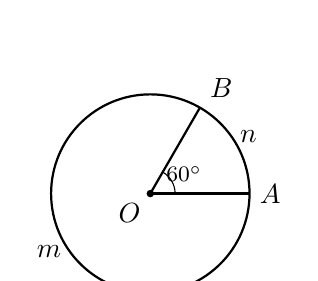
\begin{tikzpicture}[scale=0.9]
  \coordinate (O) at (0,0);
  \draw[thick] (O) circle (1.4);
  \coordinate (A) at (1.4,0);
  \coordinate (B) at (60:1.4);
  \draw[thick] (O) -- (A) node[right]{$A$};
  \draw[thick] (O) -- (B) node[above right]{$B$};
  \fill (O) circle (1.5pt) node[below left]{$O$};
  \draw (0.35,0) arc (0:60:0.35);
  \node at (30:0.55) {\footnotesize $60^\circ$};
  \node at (30:1.6) {$n$};
  \node at (210:1.65) {$m$};
\end{tikzpicture}
\end{center}
\choice
{$120^\circ$ và $300^\circ$}
{$60^\circ$ và $60^\circ$}
{\True $60^\circ$ và $300^\circ$}
{$60^\circ$ và $120^\circ$}
\loigiai{
Góc ở tâm $\widehat{AOB} = 60^\circ$ chắn cung nhỏ $AnB$ nên $\text{sđ}\wideparen{AnB} = 60^\circ$. Số đo cung lớn $AmB$ bằng $360^\circ - 60^\circ = 300^\circ$.
}
\end{ex}

\begin{ex}
Một cột đèn có bóng trên mặt đất dài $7{,}2\text{ m}$. Các tia nắng mặt trời tạo với mặt đất một góc xấp xỉ $42^\circ$. Chiều cao xấp xỉ của cột đèn là:
\begin{center}
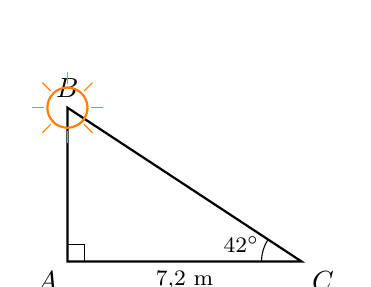
\begin{tikzpicture}[scale=0.85]
  \coordinate (A) at (0,0);
  \coordinate (B) at (0,2.3);
  \coordinate (C) at (3.5,0);
  \draw[thick] (A) -- (B) node[above]{$B$} -- (C) node[below right]{$C$} -- cycle;
  \node[below left] at (A) {$A$};
  \draw (A) ++(0,0.25) -- ++(0.25,0) -- ++(0,-0.25);
  \draw (C) ++(-0.6,0) arc (180:146:0.6);
  \node at (2.6,0.25) {\footnotesize $42^\circ$};
  \node[below] at (1.75,0) {\footnotesize $7{,}2\text{ m}$};
  \draw[orange, thick] (B) circle (0.3);
  \foreach \ang in {0, 45, 90, 135, 180, 225, 270, 315} {
    \draw[orange, thin] (B) ++(\ang:0.35) -- ++(\ang:0.18);
  }
\end{tikzpicture}
\end{center}
\choice
{\True $6{,}48\text{ m}$}
{$8\text{ m}$}
{$4{,}82\text{ m}$}
{$5{,}35\text{ m}$}
\loigiai{
Gọi $h$ là chiều cao cột đèn. Áp dụng tỉ số lượng giác trong tam giác vuông: $h = 7{,}2 \cdot \tan 42^\circ \approx 7{,}2 \cdot 0{,}9004 \approx 6{,}48\text{ m}$.
}
\end{ex}

\begin{ex}
Kết quả rút gọn của biểu thức $\sqrt[3]{8} + \sqrt[3]{-27} + \sqrt[3]{-64}$ là:
\choice
{$5$}
{\True $-5$}
{$9$}
{$-9$}
\loigiai{
Ta có $\sqrt[3]{8} = 2$, $\sqrt[3]{-27} = -3$, $\sqrt[3]{-64} = -4$. Thay vào biểu thức: $2 + (-3) + (-4) = -5$.
}
\end{ex}

\begin{ex}
Cho tam giác $MNE$ vuông tại $M$, đường cao $MH$. Hệ thức nào sau đây là đúng?
\choice
{\True $\frac{1}{MH^2} = \frac{1}{MN^2} + \frac{1}{ME^2}$}
{$MH^2 = MN^2 + ME^2$}
{$\frac{1}{MH} = \frac{1}{MN} + \frac{1}{ME}$}
{$MH^2 = NE \cdot HE$}
\loigiai{
Theo hệ thức lượng trong tam giác vuông, nghịch đảo bình phương đường cao ứng với cạnh huyền bằng tổng các nghịch đảo bình phương của hai cạnh góc vuông: $\frac{1}{MH^2} = \frac{1}{MN^2} + \frac{1}{ME^2}$.
}
\end{ex}

\begin{ex}
Cho tam giác $ABC$ vuông tại $A$, đường cao $AH$, có $AB = 12\text{ cm}, BC = 20\text{ cm}$. Độ dài $BH, CH$ lần lượt là:
\choice
{$BH = 7{,}2\text{ cm}; CH = 11{,}8\text{ cm}$}
{$BH = 9{,}2\text{ cm}; CH = 10{,}8\text{ cm}$}
{\True $BH = 7{,}2\text{ cm}; CH = 12{,}8\text{ cm}$}
{$BH = 7{,}2\text{ cm}; CH = 12\text{ cm}$}
\loigiai{
Áp dụng hệ thức lượng $AB^2 = BH \cdot BC \implies BH = \frac{AB^2}{BC} = \frac{12^2}{20} = \frac{144}{20} = 7{,}2\text{ cm}$. Khi đó $CH = BC - BH = 20 - 7{,}2 = 12{,}8\text{ cm}$.
}
\end{ex}


\newpage
\noindent\textbf{\large PHẦN II. CÂU TRẮC NGHIỆM ĐÚNG SAI}
\vspace{1mm}
\begin{ex}
Cho bất đẳng thức $a > b$. Xét tính Đúng/Sai của các khẳng định sau:
\choiceTF
{\True $a - 4 > b - 4$.}
{$-3a > -3b$.}
{\True $-2a + 3 < -2b + 3$.}
{\True $5a - 1 > 5b - 2$.}
\loigiai{
\begin{itemize}[leftmargin=*]
  \item a) Đúng. Cộng cả hai vế của bất đẳng thức $a > b$ với $-4$ ta được $a - 4 > b - 4$.
  \item b) Sai. Nhân cả hai vế của $a > b$ với số âm $-3$ thì bất đẳng thức đổi chiều: $-3a < -3b$. Do đó khẳng định này Sai.
  \item c) Đúng. Vì $a > b \implies -2a < -2b \implies -2a + 3 < -2b + 3$. Do đó khẳng định này Đúng.
  \item d) Đúng. Vì $a > b \implies 5a > 5b$. Lại có $-1 > -2$. Cộng từng vế hai bất đẳng thức cùng chiều: $5a - 1 > 5b - 2$. Do đó khẳng định này Đúng.
\end{itemize}
}
\end{ex}

\begin{ex}
Cho tam giác $ABC$ vuông tại $A$, đường cao $AH$. Biết $AC = 6\text{ cm}, BC = 10\text{ cm}$. Xét tính Đúng/Sai của các khẳng định sau:
\choiceTF
{\True $\sin B = \frac{3}{5}$.}
{$\tan C = \frac{3}{4}$.}
{\True $AH = 4{,}8\text{ cm}$.}
{Chu vi của tam giác $ABH$ bằng $14{,}4\text{ cm}$.}
\loigiai{
\begin{itemize}[leftmargin=*]
  \item a) Đúng. Ta có $\sin B = \frac{AC}{BC} = \frac{6}{10} = \frac{3}{5}$. Khẳng định Đúng.
  \item b) Sai. Áp dụng định lí Pythagore: $AB = \sqrt{BC^2 - AC^2} = \sqrt{10^2 - 6^2} = 8\text{ cm}$. Khi đó $\tan C = \frac{AB}{AC} = \frac{8}{6} = \frac{4}{3} \neq \frac{3}{4}$. Khẳng định Sai.
  \item c) Đúng. Áp dụng hệ thức lượng $AH \cdot BC = AB \cdot AC \implies AH = \frac{8 \cdot 6}{10} = 4{,}8\text{ cm}$. Khẳng định Đúng.
  \item d) Sai. Ta có $BH = \frac{AB^2}{BC} = \frac{8^2}{10} = 6{,}4\text{ cm}$. Chu vi tam giác $ABH$ bằng $AB + BH + AH = 8 + 6{,}4 + 4{,}8 = 19{,}2\text{ cm} \neq 14{,}4\text{ cm}$. Khẳng định Sai.
\end{itemize}
}
\end{ex}


\vspace{2mm}
\noindent\textbf{\large PHẦN III. CÂU TRẢ LỜI NGẮN}
\vspace{1mm}
\begin{ex}
Trong các phương trình sau:\par (1) $3\sqrt{y} - 2x = 0$; \quad (2) $2x + y = 0$; \quad (3) $x^2 - y^2 = 12$; \quad (4) $2x + y + 3z = 0$.\par Phương trình bậc nhất hai ẩn là phương trình số mấy?
\shortans{Phương trình (2)}
\loigiai{
Phương trình bậc nhất hai ẩn có dạng $ax + by = c$ ($a, b$ không đồng thời bằng 0). Do đó chỉ có phương trình (2) thỏa mãn.
}
\end{ex}

\begin{ex}
Cho tam giác $ABC$ vuông tại $A$, biết $AB = 12\text{ cm}, AC = 9\text{ cm}, BC = 15\text{ cm}$. Tính số đo góc $B$ (làm tròn đến độ).
\shortans{$37^\circ$}
\loigiai{
Xét tam giác $ABC$ vuông tại $A$, ta có $\cos B = \frac{AB}{BC} = \frac{12}{15} = 0{,}8$. Suy ra $\widehat{B} = \arccos(0{,}8) \approx 37^\circ$.
}
\end{ex}


\newpage
\noindent\textbf{\large PHẦN IV. TỰ LUẬN}
\vspace{1mm}
\noindent\textbf{Câu 1 (2,0 điểm).}

Giải các phương trình và hệ phương trình sau:\par a) $(4x + 5)(3x - 2) = 0$.\par b) $\frac{4}{x(x - 1)} + \frac{3}{x} = \frac{4}{x - 1}$.\par c) $\begin{cases} x - 3y = 4 \\ -2x + 6y = -8. \end{cases}$

\noindent\textbf{Lời giải:}

a) $(4x + 5)(3x - 2) = 0 \iff 4x + 5 = 0$ hoặc $3x - 2 = 0 \iff x = -\frac{5}{4}$ hoặc $x = \frac{2}{3}$.\par Vậy tập nghiệm của phương trình là $S = \left\{-\frac{5}{4}; \frac{2}{3}\right\}$.\par b) Điều kiện xác định: $x \neq 0$ và $x \neq 1$.\par Quy đồng mẫu thức chung $x(x - 1)$ và khử mẫu:\par $4 + 3(x - 1) = 4x \iff 4 + 3x - 3 = 4x \iff 3x + 1 = 4x \iff x = 1$ (không thỏa mãn ĐKXĐ).\par Vậy phương trình vô nghiệm.\par c) $\begin{cases} x - 3y = 4 \quad (1) \\ -2x + 6y = -8 \quad (2) \end{cases}$\par Nhân hai vế của phương trình (1) với 2 ta được: $\begin{cases} 2x - 6y = 8 \\ -2x + 6y = -8 \end{cases}$\par Cộng vế theo vế hai phương trình ta được $0x + 0y = 0$ (luôn đúng với mọi $x, y$).\par Vậy hệ phương trình có vô số nghiệm với nghiệm tổng quát: $\left(x; \frac{x - 4}{3}\right)$ với $x \in \mathbb{R}$.

\vspace{3mm}
\noindent\textbf{Câu 2 (1,5 điểm).}

Người ta cho thêm $1\text{ kg}$ nước vào dung dịch $A$ (chứa axit $X$) thì được dung dịch $B$ có nồng độ axit là $20\%$. Sau đó lại cho thêm $1\text{ kg}$ axit $X$ vào dung dịch $B$ thì được dung dịch $C$ có nồng độ axit là $33\frac{1}{3}\%$. Tính nồng độ axit của dung dịch $A$ ban đầu.

\noindent\textbf{Lời giải:}

Gọi khối lượng dung dịch $A$ là $x\text{ (kg)}$ và khối lượng axit nguyên chất là $y\text{ (kg)}$ ($x > y > 0$).\par Khi thêm $1\text{ kg}$ nước, khối lượng dung dịch $B$ là $x + 1\text{ (kg)}$. Nồng độ axit trong $B$ là $20\%$ nên:\par $\frac{y}{x + 1} = 20\% = \frac{1}{5} \implies x + 1 = 5y \iff x - 5y = -1 \quad (1)$\par Khi thêm tiếp $1\text{ kg}$ axit vào dung dịch $B$, khối lượng axit là $y + 1\text{ (kg)}$ và khối lượng dung dịch $C$ là $x + 1 + 1 = x + 2\text{ (kg)}$. Nồng độ dung dịch $C$ là $33\frac{1}{3}\% = \frac{1}{3}$ nên:\par $\frac{y + 1}{x + 2} = \frac{1}{3} \implies 3(y + 1) = x + 2 \iff x - 3y = 1 \quad (2)$\par Từ (1) và (2) ta có hệ phương trình: $\begin{cases} x - 5y = -1 \\ x - 3y = 1 \end{cases}$\par Lấy phương trình thứ hai trừ phương trình thứ nhất vế theo vế ta được: $2y = 2 \implies y = 1$ (kg).\par Thay $y = 1$ vào (2): $x = 3(1) + 1 = 4$ (kg) (thỏa mãn điều kiện).\par Nồng độ axit của dung dịch $A$ ban đầu là: $\frac{y}{x} = \frac{1}{4} = 25\%$.\par Vậy nồng độ axit của dung dịch $A$ là $25\%$.

\vspace{3mm}
\newpage
\noindent\textbf{Câu 3 (1,0 điểm).}

Một cầu trượt trong công viên có độ dốc là $28^\circ$ và có độ cao là $2{,}1\text{ m}$. Tính độ dài của mặt cầu trượt (làm tròn đến chữ số thập phân thứ nhất).
\begin{center}
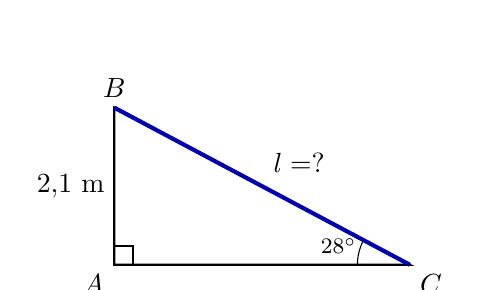
\begin{tikzpicture}[scale=0.95]
  \coordinate (A) at (0,0);
  \coordinate (B) at (0,2.1);
  \coordinate (C) at (3.95,0);
  \draw[thick] (A) node[below left]{$A$} -- (B) node[above]{$B$} -- (C) node[below right]{$C$} -- cycle;
  \draw (A) ++(0,0.25) -- ++(0.25,0) -- ++(0,-0.25);
  \draw (C) ++(-0.7,0) arc (180:152:0.7);
  \node at (3.0,0.25) {\footnotesize $28^\circ$};
  \node[left] at (0,1.05) {$2{,}1\text{ m}$};
  \node[above right] at (2.0,1.1) {$l = ?$};
  \draw[line width=1.5pt, blue!70!black] (B) -- (C);
\end{tikzpicture}
\end{center}

\noindent\textbf{Lời giải:}

Mô hình hóa bài toán bằng tam giác $ABC$ vuông tại $A$, trong đó:\par - $AB$ là chiều cao của cầu trượt: $AB = 2{,}1\text{ m}$.\par - Góc nghiêng dốc của cầu trượt là góc nhọn $\widehat{C} = 28^\circ$.\par - $BC$ là độ dài của mặt cầu trượt (cạnh huyền).\par Xét tam giác $ABC$ vuông tại $A$, ta có:\par $\sin C = \frac{AB}{BC} \implies BC = \frac{AB}{\sin C} = \frac{2{,}1}{\sin 28^\circ} \approx \frac{2{,}1}{0{,}4695} \approx 4{,}47\text{ m}$.\par Làm tròn đến chữ số thập phân thứ nhất, độ dài của mặt cầu trượt khoảng $4{,}5\text{ m}$.

\vspace{3mm}
\noindent\textbf{Câu 4 (0,5 điểm).}

Cho tam giác $ABC$ vuông tại $A$. Chứng minh rằng $\sin^2 B + \sin^2 C = 1$.

\noindent\textbf{Lời giải:}

Trong tam giác $ABC$ vuông tại $A$, hai góc nhọn $B$ và $C$ phụ nhau, tức là $\widehat{B} + \widehat{C} = 90^\circ$.\par Theo tính chất tỉ số lượng giác của hai góc phụ nhau, ta có: $\sin C = \cos B$.\par Thay vào vế trái của biểu thức ta được:\par $\sin^2 B + \sin^2 C = \sin^2 B + \cos^2 B$.\par Mặt khác, theo định nghĩa tỉ số lượng giác trong tam giác vuông $ABC$:\par $\sin B = \frac{AC}{BC},\; \cos B = \frac{AB}{BC} \implies \sin^2 B + \cos^2 B = \frac{AC^2 + AB^2}{BC^2}$.\par Áp dụng định lí Pythagore: $AB^2 + AC^2 = BC^2$, suy ra:\par $\sin^2 B + \cos^2 B = \frac{BC^2}{BC^2} = 1$.\par Vậy $\sin^2 B + \sin^2 C = 1$ (đpcm).

\vspace{3mm}

\vfill
\begin{center}
  \textbf{--- HẾT ---}
\end{center}
\end{document}
